\usepackage[utf8]{inputenc}
\usepackage{array}
\documentclass[12pt]{report}

% Bar chart drawing library 
\usepackage{pgfplots} 
% Curve


\usepackage{graphicx}
\graphicspath{ {./images/} }
\usepackage{pgfgantt}
\usepackage[a4paper, total={7in, 10in}]{geometry}


\title{A Comprehensive Guide to the History and Solutions to the Brachistochrone Problem: EPQ Report}
\author{Zayaan Mulla}
\date{December 2021}

\begin{document}

\maketitle

\tableofcontents
\chapter{Abstract}
The first time I heard of the Brachistochrone Problem was in class, through my teacher. He was telling us about a problem set by one of the Bernoulli brothers, in order to entice Newton into coming out of retirement. The problem was to find the curve of fastest descent, or more commonly known as the Brachistochrone Problem.
\\
\\
Having set out to find out more about the 'curve of fastest descent', I discovered Fermat's Principle, and and how Johann Bernoulli utilised it in solving the Brachistochrone Problem. I also came across the Calculus of Variations and the Euler-Lagrange Equation, which through the Beltrami Identity, provided basis for an elegant proof to the problem. Due to the wide array of topics I would be exposed to, I hence concluded that my topic of choice for my EPQ should be centred around the Brachistochrone problem, and should form an introduction to the solutions to the problem, as well as its fascinating history.
\\
\\
The purpose of the project is to present the, otherwise inaccessible, mathematics of the problem in a more accessible form through a guide, such that it can be read and understood by an advanced high school student who has studied calculus. Over the course of the Guide, we will go over the history of the Brachistochrone Problem, and look over the mathematicians that solved it. We will also examine the approaches taken to solving the problem, from the ingenious proof using Fermat's Principle and Snell's Law by Johann Bernoulli, to the more rigorous method of the Calculus of Variations developed by Leonhard Euler. I will attempt to prove most of the results I mention in attempt to be thorough, but I also hope that the Guide is comprehensible and fascinating to the majority. The EPQ has also given me the opportunity to learn LATEX, the software which this Guide is written in, which will be invaluable when studying Mathematics at University next year. The Pre-Requisites in order to understand the Guide involve understanding Calculus up until A-Level, a brief understanding of Partial Derivatives and the Multivariable Chain Rule, familiarity with Trignometry, some intuition for Physics, and most importantly, an interest in the topic and motivation to learn. I hope you enjoy!
\\
\\
Zayaan

\chapter{Aims, Purpose, and Target Audience}
Throughout year 12 and 13, despite a large amount of the subject of physics being based on Newton's Calculus (especially the physics covered at A-Level), I have noticed a distinct lack of Calculus based physics presented throughout the A-Level Physics course. It is for this reason I decided to ensure my project delves deeper into the applications of Calculus in physics, and uncovers the vast powers of calculus on solving seemingly trivial problems such as the Brachistochrone.
\\
\\
My project however is based on a specific part of Calculus, or more specifically a derivative of calculus itself, the Calculus of Variations, which was originally developed by the famous Mathematician Leonhard Euler. Rather than find the stationary points of a function such as in differential calculus, its aim to find the stationary functions of a functional, and hence is perfect for solving a problem such as this. The project will hopefully widen the horizons of current A-Level Physics students, the majority of which take Mathematics to A-Level as well, who have been exposed to Calculus before at an elementary level. Through the project they will be able to gain a new insight into the wider applications of Calculus through a more interesting, well defined problem of which they have been provided context for.
\\
\\
Topics in A-Level Physics such as Snell's Law, which were not proven in the syllabus, or given any context for in terms of the motivations behind the law will also be proven rigorously, and be explained carefully through fundamental principles. The project will aim to further patch gaps in the readers understanding of equations simply provided to them at A-Level, and will build upon them to prove more complex results without a loss of generality.
\\
\\
Furthermore, due to the target audience of the project being highly skilled mathematicians, who are preferably taking Further Mathematics to A-Level as well, another purpose of the guide will be to introduce them to more advanced techniques in problem solving, such as multivariate calculus, and fascinatingly, Leibniz rule, which is an extremely powerful method of solving seemingly impossible integrals. This again covers the gap in the A-Level syllabus in terms of advanced problem solving techniques, which should catered to more advanced individuals, mathematically speaking.
\\
\\
To summarize, we can clearly define the aims, and success criteria of the project to be:
\\
\\
\begin{itemize}
    \item Ensure all non trivial equations are derived appropriately
    \item Explain motivations behind equations and mathematics conducted
    \item Provide an introduction to advanced problem solving techniques in Calculus and geometry
    \item Cover the gaps in the A-Level syllabus in terms of completeness, relevant to the project
    \item Provide historical context
\end{itemize}

\chapter{Data Collection}
Although I would have preferred to base my EPQ on the Brachistochrone problem, one of the reasons I decided to pursue an EPQ was to spread the joy I get in learning different Mathematical concepts to others. Therefore, I produced a poll using google forms to be submitted by maths students at DESC regarding which topic I should pursue from my list of initial ideas in order to find out the preference of my intended audience. The poll consisted of options in Graph Theory and Euler's Polyhedron Formula which is of a more discrete nature and The Brachistochrone Problem. The results of the poll, shown below, suggested that the Brachistochrone Problem was the most popular option, and hence formed the basis of my EPQ.
\\
\\
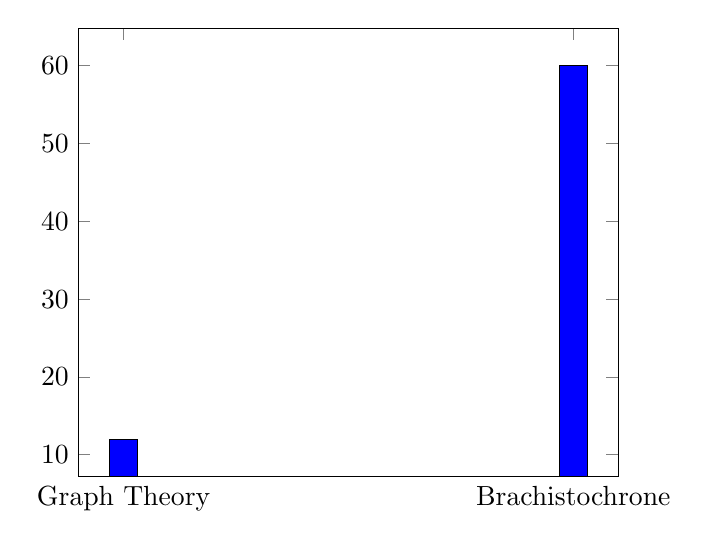
\begin{tikzpicture}
        \begin{axis}[
            symbolic x coords={Graph Theory, Brachistochrone},
            xtick=data
          ]
            \addplot[ybar,fill=blue] coordinates {
                (Graph Theory,   12)
                (Brachistochrone,   60)
            };
        \end{axis}
\end{tikzpicture}
\\
\\
Another decision I contemplated over was the format in which to present my project. One of the Objectives of the EPQ is to ensure that it is well understood by the target audience, which is why I decided to present that target audience with another poll through google forms. The options were either a text based guide, where I would present the mathematics line by line with my explanations to the contents in text, or a 50/50 split between text and video explanations where detailed mathematical proof is present. The results of the poll favoured the former option as demonstrated by the chart below.
\\
\\
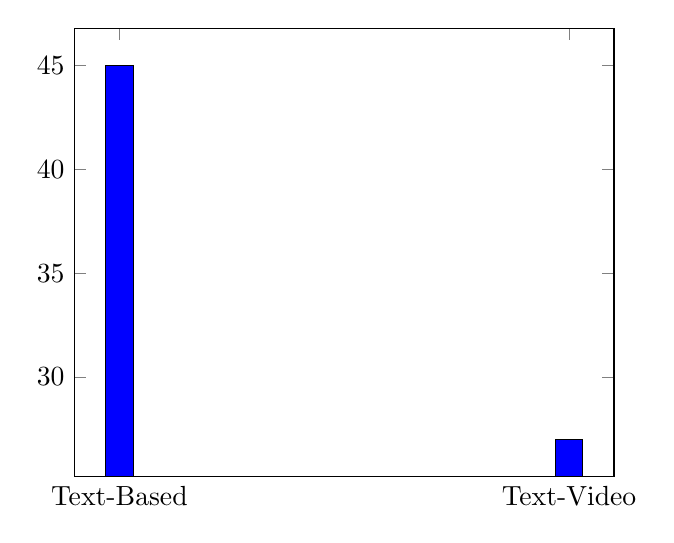
\begin{tikzpicture}
        \begin{axis}[
            symbolic x coords={Text-Based, Text-Video},
            xtick=data
          ]
            \addplot[ybar,fill=blue] coordinates {
                (Text-Based,   45)
                (Text-Video, 27)
                
            };
        \end{axis}
\end{tikzpicture}

\chapter{Planning Work - Gantt Chart}
\\
\\
The tasks needed to complete the project (Exact resources used detailed in logbook) can be summarized in the following list, with their timeline conveyed through the Gantt chart below:
\begin{enumerate}
    \item Compile full list of resources and items to be used as reference within the project, complete surveys on topic choice and method of delivering content
    
    \item Complete intro to calculus of variations
    
    \item In order to implement the recommendation by my coordinator to use videos to convey the content I will be presenting, I will use blog link to teach myself the basics of Imovie video editing, Further familiarise myself with writing mathematics through Latex via wiki link
    \\
    \\
    \(\star\) note that the idea of conveying the mathematics through video form was later discarded
    
    \item Using the current list of initial resources (more may be added by the time I complete this task) complete the first subchapter on introduction to the brachistochrone problem and state the motivations of the guide and present an intuitive approach to understanding the problem as well as brief context behind it
    
    \item Compile historical account of the brachistochrone problem for the second subchapter (A brief history)
    
    \item Begin work on creating videos for the following topics as well as teaching them to yourself and ensure understanding first before doing so to provide a clear explanation : Deriving snell’s Law, The Parametric equations of a cycloid, * edit: use mark levi’s insight to how parametric equations of a cycloid relate to snells law to provide context
    \\
    \\
    \(\star\) note the videos mentioned were later converted to text based explanations
    
    \item write up subchapters on each of the topics mentioned above and complete references for each
    
    \item combine work on previous subchapters to use in presenting fermats proof. record video and edit. Write up subchapters and provide historical context for fermats proof.
    
    \item refamiliarize yourself of calculus of variations through the following video: https://www.youtube.com/watch?v=VCHFCXgYdvY&t=360s, Complete subchapter on the introduction to the calculus of variations, and give mathematical, as well as historical context to the topic
    
    \item complete video on deriving the Euler-Lagrange equation *edit: as well as providing an example through the shortest distance path problem. Proof and edit the videos and write up subchapters on both topics.
    \\
    \\
    \(\star\) note the videos mentioned were later converted to text based explanations
    
    \item Complete explanation on solving the brachistochrone problem via the calculus of variations and complete subchapter containing context. Derive the beltrami identity for completeness. * edit: deriving the beltrami identity should be in its own subchapter.
    
    \item proof entire document as well as videos. Complete side report containing survey data analysis and source analysis as well as an initial abstract on the topic. * edit: Trial product with 2 member of my maths class and collect feedback – present this feedback in 1000 word side report. 
    
    \item produce presentation along with script
    \item trial presentation and give it to class
    
    \item complete logbook and submit project


\end{enumerate}


\begin{figure}[tbp]
\begin{center}

\begin{ganttchart}[y unit title=0.4cm,
y unit chart=0.5cm,
vgrid,hgrid, 
title label anchor/.style={below=-1.6ex},
title left shift=.05,
title right shift=-.05,
title height=1,
progress label text={},
bar height=0.7,
group right shift=0,
group top shift=.6,
group height=.3]{1}{24}
%labels
\gantttitle{Date}{24} \\
\gantttitle{July: 1-15}{4} 
\gantttitle{July: 16-30}{4} 
\gantttitle{Aug: 1-15}{4} 
\gantttitle{Aug: 16-30}{4} 
\gantttitle{Sept: 1-15}{4} 
\gantttitle{Sept: 16-30}{4} \\
%tasks
\ganttbar{task 1}{1}{4} \\
\ganttbar{task 2}{5}{8} \\
\ganttbar{task 3}{9}{12} \\
\ganttbar{task 4}{13}{16} \\
\ganttbar{task 5}{17}{20} \\
\ganttbar{task 6}{21}{24} 



\end{ganttchart}
\end{center}
\end{figure}

\begin{figure}[tbp]
\begin{center}

\begin{ganttchart}[y unit title=0.4cm,
y unit chart=0.5cm,
vgrid,hgrid, 
title label anchor/.style={below=-1.6ex},
title left shift=.05,
title right shift=-.05,
title height=1,
progress label text={},
bar height=0.7,
group right shift=0,
group top shift=.6,
group height=.3]{1}{24}
%labels
\gantttitle{Date}{24} \\
\gantttitle{Oct: 1-15}{4} 
\gantttitle{Oct: 16-30}{4} 
\gantttitle{Nov: 1-15}{4} 
\gantttitle{Nov: 16-30}{4} 
\gantttitle{Dec: 1-15}{4} 
\gantttitle{Dec: 16-30}{4} \\
%tasks
\ganttbar{task 7}{1}{4} \\
\ganttbar{task 8}{5}{8} \\
\ganttbar{task 9}{9}{12} \\
\ganttbar{task 10}{13}{16} \\
\ganttbar{task 11}{17}{20} \\
\ganttbar{task 12}{21}{24} 


\end{ganttchart}
\end{center}
\end{figure}

\begin{figure}[tbp]
\begin{center}

\begin{ganttchart}[y unit title=0.4cm,
y unit chart=0.5cm,
vgrid,hgrid, 
title label anchor/.style={below=-1.6ex},
title left shift=.05,
title right shift=-.05,
title height=1,
progress label text={},
bar height=0.7,
group right shift=0,
group top shift=.6,
group height=.3]{1}{24}
%labels
\gantttitle{Date}{24} \\
\gantttitle{January}{8} 
\gantttitle{February}{8} 
\gantttitle{March}{8} \\

%tasks
\ganttbar{task 13}{1}{8} \\
\ganttbar{task 14}{9}{16} \\
\ganttbar{task 15}{17}{24} \\



\end{ganttchart}
\end{center}
\end{figure}


\chapter{Production Process}
The Production process begun by researching the history of the Brachistochrone problem, and how the problem originated, including who solved it. The source I found most useful here was [1]. I proceeded to write an account of my findings in the first chapter of the project, drawing on Galileo's initial attempt, and proceeding to explain the involvement of the Bernoulli brothers, culminating in Newton's remarkable attempt on solving the problem. 
\\
\\
The next stage in my preliminary research was to find the solution to the problem itself. This is where I came across the fact that this problem was solved primarily using three different methods. Firstly, the analytical method that led to a differential equation which would unveil the parametric equations of a cycloid, the solution to the Brachistochrone problem. This method was employed by Johann Bernoulli, the first to solve the problem. Secondly, the solution through the Calculus of Variations, and more specifically the Euler-Largrange equation. This was the method that particularly peaked my interest in the Brachistochrone problem itself, as it displayed perfectly the use of complex mathematics, to solve a seemingly simple problem, such as that used in Andrew Wiles' proof of Fermat's Last Theorem, obviously at a significantly smaller scale. The third method was a computation involving the use of numerical solutions, such as Euler's method and the Newton-Raphson approximation. Due to my disinterest however in computer based proofs, I decided to exclude this from the project as I felt that it would ruin the mathematical preciseness of the project itself. Furthermore, due to the negative reactions from the mathematical community to other computer assisted proofs, such as the one of the four colour theorem, I decided that it would be best to avoid the topic altogether as we already had other mathematical proofs, more rich in history and mathematics itself, than the ones assisted by the computer.
\\
\\
The next stage of the production was to decide on the title, and contents of the guide. I decided to title the project 'A Comprehensive Guide to the History and Solutions to the Brachistochrone Problem', as I felt that it best encapsulated the contents of the project itself. In terms of the contents, I decided to divide the project up into three main sections, An introduction to the problem itself, covering a brief history of the problem, as well as an in depth explanation of the problem statement. The second section was to cover the analytical solution of the problem, going over the derivation of Snell's Law from Fermat's principle of least time, as well as presenting the motivations behind the parametric equations of the cycloid and modern geometrical proof of them, before culminating in Johann Bernoulli's proof.
The final chapter would go over The Calculus of Variations, and begin from first principles by deriving the Euler-Lagrange Equation, and demonstrating its applications through a simpler problem before using it fully to compute the solution to the Brachistochrone problem.
\\
\\
What I felt made this project more than simply copying mathematical proofs from the internet was the way the proofs were presented. Sources online, as well as those used as references in this project, I discovered to be far too inaccessible to the average user, and in turn would prevent many from discovering the actual mathematics used in solving this famous problem. The way I intended to present the mathematics was by ensuring that I understood the solutions completely, before presenting them in my own style, carefully justifying each step in the mathematics conducted throughout to ensure that it is not overwhelming to comprehend nor confusing in any way to the reader.
\\
\\
Upon deciding the list of topics, I produced a list of sources, approximately two targeted at each subsection to draw from. This was then shortened to contain only essential references so that I would only use them for the sake of inspiration rather than a source from which a whole section is simply taken from. I then proceeded to take notes from the sources using pen and paper in a single dedicated textbook, on each individual topic, and formulate them in such a way that the notes could be easily translated onto the final document. I also added in my own explanations and little ideas to better present the proof into this book so that when I get to compiling the guide it would be a smooth process.
\\
\\
Some problems I faced in analysing the sources were a lack of knowledge in certain areas of undergraduate mathematics, such as multivariate calculus. I then realised that in order to understand the mathematics of the project in detail, so that I could present it well to a reader such that they required minimal pre-requisite knowledge, I would need to understand the pre-requisite knowledge for myself. This is when I decided to watch and work on the MIT OCW multivariate calculus course. Completing this course was extremely valuable not only to this project, but to my own mathematical maturity, and was a particularly interesting topic to learn due to its vast amount of applications. Another distinct lack of knowledge I found was in the area of solving differential equations, and advanced techniques in integration. I filled in these gaps by reading over the A-Level Further Maths CP2 chapter on differential equations early, as well as learning some more advanced topics in integration such as Leibniz rule, indefinite integrals, integration through substitution involving hyperbolic functions, and lastly the reduction formula from FP2 in A-Level Further Maths. Despite not utilising all of this mathematics individually, the maturity gained mathematically from self teaching all of these topics, as well as the ability to now comprehend more advanced sources of information was invaluable in completing the project as a whole.
\\
\\
Despite my initial idea being to create individual videos on each topic, I decided against this as, upon feedback from my classmates who are my intended audience, I concluded that they would prefer a text based approach. This was mainly due to videos taking up unnecessary time in explaining a solution, whereas they would be able to read a document much faster and make sense of it easier if they were to evaluate it themselves, rather than through a spokesperson.
\\
\\
Having decided the format of the project, it was now time to implement the first draft through LATEX. I decided to use LATEX software through overleaf due to its reliability, given that it is used my various major educational institutes including Caltech. Furthermore, LATEX gave the opportunity to communicate the mathematics easily through code, and also gave me the option of installing multiple TEX based packages such as 'amsmaths' and 'pgfplots' for stunning diagrams and presentation of the mathematics as a whole. All in all the use of LATEX software also ensured that I would gain a valuable skill in typesetting as I go to university next year to study a degree in Mathematics.
\\
\\
After implementing the project, I had it proofreading it several times for errors, I decdided that the best way to test whether or not the project was a success was to trial it with members of my maths class. Their feedback is contained within this same report however it can be summarized to say that the project met all the success criteria outlined initially. I then proceeded to set aside development of the project itself and went onto work on the project logbook and this report itself.


\chapter{Evaluation of Product}

Upon suggestion from my supervisor I asked 2 members of my target audience to produce an evaluation of the guide, which enabled me to measure its success with respect to its intended consumers. The evaluation report was co-written by Misha Melnichuk and Matias De Araujo, both members of my Further Maths class.
\begin{itemize}
    \item Chapter 1: Introduction to the Brachistochrone Problem (Misha Melnichuk)
    \\
    \\
    "I believe that the section on stating the Brachistochrone problem was concise and to the point. The diagram also helped visualise the problem which was useful for building some intuition for the problem. The second section of the chapter was on the history of the problem. I particularly enjoyed this part as this caused me to develop a firm interest in how the solution to the problem would unfold. It was truly fascinating how the section developed from going over Galileo's work on the problem to Johann Bernoulli using the problem as a challenge to Newton, and how his solution was to show he was the best Mathematician of his generation. The plot of Newton's story in regards to the problem was well developed and was of sufficient detail to not only causing the readers interest to spike, but to ensure it is retained due to its lack of irrelevant information."
    \item Chapter 2: Johann Bernoulli and Fermat's Principle (Misha Melnichuk)
    \\
    \\
    "The first section of Deriving Snell's Law was useful to go over as it helped provide some background information when going over Bernoulli's proof. Furthermore, it enabled me to grow my knowledge of a topic that was introduced in A-Level Physics, and to gain a more solid understanding of the mathematics behind Snell's Law which was extremely interesting, and would be for any mathematically inclined A-Level Physics student. The same goes for the Parametric equations of a Cycloid. Although I have not been exposed to it before, it was extremely useful when being presented with Bernoulli's proof as it enabled me to spot the solution when we got there, providing me with a great 'Aha!' moment, which was extremely satisfying. I believe the idea of presenting the details of the proof before tying it up together at the end was brilliant and made for an introduction to the Brachistochrone problem that was far easier to follow for a reader with no experience in the topic, such as myself."
    \\
    \\
    \item Chapter 3: The Calculus of Variations (Matias De Araujo)
    \\
    \\
    "This was the most technical chapter of the guide but turned out to be the most mathematically intriguing. The first section on the motivations of the Calculus of Variations was essential to ensuring that I understood the fundamental purpose of the topic: to find the function that minimises a functional. It also helped provide a framework to the how the Calculus of Variations came about in the first place by going over its history in Euler's collaboration with Lagrange, as well as through an example by stating the Brachistochrone problem mathematically and using that to demonstrate a general function the Calculus of Variations looks to minimise. The video explanations to the derivation of the Euler-Lagrange equation, the path of shortest distance, and the rest of the sections in this chapter were concise, yet were thorough in explaining the details of each of the topics clearly for the reader to understand, and were a key part in ensuring that the guide is comprehensible to beginners to the topic such as myself." 
\end{itemize}

\chapter{Presentation}

The details of the contents presented on each slide are contained within the logbook, however the slides will be contained below for the sake of reference.
\\
\\
\includegraphics[width=6cm, height=5cm]{EPQ - VC/Presentation/S1.jpg}
\includegraphics[width=6cm, height=5cm]{EPQ - VC/Presentation/S2.jpg} 
\\
\includegraphics[width=6cm, height=5cm]{EPQ - VC/Presentation/S3.jpg} 
\includegraphics[width=6cm, height=5cm]{EPQ - VC/Presentation/S4.jpg} 
\\
\includegraphics[width=6cm, height=5cm]{EPQ - VC/Presentation/S5.jpg} 
\includegraphics[width=6cm, height=5cm]{EPQ - VC/Presentation/S6.jpg} 
\\
\includegraphics[width=6cm, height=5cm]{EPQ - VC/Presentation/S7.jpg} 



\chapter{Source Analysis}
\begin{itemize}
    \item [1] https://mathshistory.st-andrews.ac.uk/HistTopics/Brachistochrone/ 
    \item [2] https://tex.stackexchange.com/questions/568105/illustrating-newtons-path-of-fastest-descent
    \item [3] https://www.maa.org/press/periodicals/convergence/historical-activities-for-calculus-module-3-optimization-galileo-and-the-brachistochrone-problem
    \item [4] https://www.youtube.com/watch?v=3HXCv4dmR7A
    \item [5] http://scipp.ucsc.edu/~haber/ph5B/fermat09.pdf (1)
    \item [6] https://www.math.rug.nl/~broer/pdf/ws-ijbc.pdf (3-4)
    \item [7] https://ocw.mit.edu/courses/mathematics/18-02sc-multivariable-calculus-fall-2010/1.-vectors-and-matrices/part-c-parametric-equations-for-curves/session-17-general-parametric-equations-the-cycloid/ (Reading and Examples, 3)
    \item [8] https://mecheng.iisc.ac.in/suresh/me256/GalileoBP.pdf
    \item [9] http://www1.phys.vt.edu/~takeuchi/Tools/CSAAPT-Fall2019-takeuchi.pdf (5)
    \item [10] https://www.youtube.com/watch?v=VCHFCXgYdvY&t=348s
    \item [11] https://www.youtube.com/watch?v=YVLFHE-mJ7w
    \item [12] https://www.youtube.com/watch?v=tm17eLIObdA
    \item [13] https://aerospace.technion.ac.il/wp-content/uploads/2020/07/Full-Report-14.7.pdf
    \item [14] https://scholarworks.umt.edu/cgi/viewcontent.cgi?article=1099&context=tme#:~:text=In
    \item [15] https://tex.stackexchange.com/questions/196957/how-can-i-draw-this-cycloid-diagram-with-tikz
    \\
    \\
    The source [1] was produced by Edmund Robertson and John O'Connor of the School of Mathematics and Statistics at the University of St. Andrews, which is one of the top universities in the UK. Their contributions to the History of Mathematics have been recognised through many awards, including the Hirst prize of the London Mathematical Society. The source places a heavy emphasis on the history of the Brachistochrone problem, particularly on Galileo's premature attempts and Newton's involvement in the problem. I would say that this source is reliable due to the accolades achieved by the department itself. This is in contrast with source [8] which does indeed cover Galileo and Newton's involvement in the problem yet does not go into too much detail in regards to their contributions. The source instead focuses on Snell's Law and Fermat's principle of least time, culminating with Johann Bernoulli's Proof as the main focus of the paper. The paper was produced by the prestigious Indian institute of science, which is the leading school in India devoted to the pursuit of answers to fundamental questions in the natural sciences. This source can be assumed to be reliable as it is utilized in educating the top minds in Indian Mathematics today.
    \\
    \\
    Source [5], from a physics course at the University of Santa Barbara, is also helpful in providing an analytical proof of Snell's Law yet does not go into many of the motivations behind it such as Fermat's principle. It also does not provide a method of solving it through the calculus of variations and hence lacks completeness, yet is adequate in providing a source for a geometric proof. Due to the proof being correct, we can treat this source as reliable. Source [6] however is more useful as although the proof of Snell's Law in it is explained less thoroughly, it does a better job explaining the motivations behind it as well as how Snell's Law is actually applied in Johann Bernoulli's proof, with more comprehensive diagrams and effective historical remarks. Given that the source is from the Bernoulli Institute itself, written by Hendrik Wolter Broer, a Dutch mathematician known for contributions to the theory of nonlinear dynamical systems at the University of Gronigen, it can be assured that it is reliable. The source is also an extension to source [8] as it shows how Johann Bernoulli's solution actually relates to a cycloid, by solving the resulting differential equation, and doesn't just simply state it. Source [7] however, an MIT course handout, is what is actually used in recognising the parametric equations of a cycloid, although it is just used as a reference and not an actual derivation. Source [13] is a paper written by Ido Braun from the Israel Institute of Technology as his thesis paper, where he presents an insightful modern geometric proof of the parametric equations of a cycloid, developed by Mark Levi of the 'Mathematical Mechanic', a bestselling book in mechanics. The source can therefore be assumed as reliable. I use the proof as context for myself whilst developing the second chapter.
    \\
    \\
    Although in the form of Youtube videos rather than the traditional academic paper format presented in the last 2 paragraphs, the following sources were still effective, maybe even more so, in demonstrating the motivations, and actual mathematics behind the Calculus of Variations and its role in the Brachistochrone Problem. These videos were used in conjunction with source [6] and [13] which were considered earlier. They also provided insights into the applications of the Calculus of Variations; in source [6], the treatment wasn't as comprehensive and left solutions in the form of differential equations that needed to be solved rather than a thorough proof. The perspective was also from a more Hamiltonian standpoint rather than Lagrangian, implementing conservation laws into the solution rather than a direct proof through Lagrangian mechanics and the Euler Lagrange equation which was my focus in the EPQ. Despite this however its emphasis on the background of the cycloid made it useful even when analysing the proof through the Calculus of Variations. Source [13] was also useful due to it's presentation of Mark Levi's Cycloid proof, and how it used that when it went on to apply the Euler-Lagrange equation to solve the Brachistochrone problem. Its chronological presentation of the analysis of the problem was a source of inspiration when choosing in which order to present my project. The source also goes onto present a thorough treatment of gravitational potential inside and outside of earth through calculus, as well as applying that concept in extensions of the Brachistochrone problem such as the  problem on the surface of the earth, which although I have not presented in the project, was an interesting perspective of the problem to read about and to deepen my understanding through. This perspective also brought light to further research that could be done in the field of the Calculus of Variations, for example, applying models such as the Brachistochrone in other real world problems. Extending techniques in the Calculus of Variations is something I look forward to looking into at University as I develop my understanding of the subject
    \\
    \\
    Source [10] provides us with an effective introduction to the calculus of variations, going over its history from Newton and Leibniz to Lagrange's work on the Tautochrone problem (A variation of the Brachistochrone), the proof of the Euler-Lagrange equation, as well as emphasising how it's different to differential calculus. This source however is simply meant to develop intuition for the topic, although is meant to be a highly reputable source simply based on the views it has generated, and the overwhelming majority of comments positively appreciating the video. This source is hence one that is reliable. Source [11] was by the same creator and formed a useful demonstration of the applications of the Euler-Lagrange equation on a question we actually know the answer to. Comments such as: "Very well explained! I enjoy your calm style of presentation." and "Great video. You deserve to get a large subscriber base." were reassuring in confirming the reliability video series as an unconventional source of an EPQ project. The videos also provided a framework from which I could produce my own explanations, yet were not the only source of inspiration for my own explanations.
    \\
    \\
    Overall, the wide variety of sources I selectively made use of, from papers in academic journals to Youtube videos from enthusiastic content creators, were one of the main reasons I believe the project turned out to be a success in it's mission: to provide an effective, accessible introduction to the Brachistochrone Problem. 
    
\end{itemize}

\chapter{Use of Technology}
Despite the project being based mainly on proof based mathematics, the communication of the project was through LATEX, a document preparation system used for the communication and publication of scientific documents. LATEX is used widely throughout academia and is popular amongst scholars for its ability to easily convey mathematical expressions through code. It is based off, and is comprised of TEX macros.
\\
\\
I further utilized the TikZ package withing LATEX in order to produce the graphical elements in the project, such as the diagram I used to demonstrate that \(ds = \sqrt{dx^2+dy^2}\)
The instructions on using the package are detailed at https://www.overleaf.com/learn/latex/TikZpackage.
\\
\\
Another package I used within the LATEX software was Pgfplots, which allowed me graph complex functions efficiently, with maximal customization features such as the distinction between dotted and smooth curves, and the colouring and identification of curves through legends, in order to make the functions explicit. Despite not having used them, in addition to two dimensional functions, the package is powerful enough to graph three dimensional functions as well, making it extremely popular throughout academic publishing. The instructions on using the package are detailed at https://www.overleaf.com/learn/latex/Pgfplotspackage.


 


\end{document}
